\documentclass[10pt]{article}

\usepackage[T1]{fontenc}
\usepackage{microtype}
\usepackage[margin=0.78in]{geometry}
\usepackage{booktabs}
\usepackage{tabularx}
\usepackage{array}
\usepackage{amsmath}
\usepackage{xcolor}
\usepackage{graphicx}
\usepackage{tikz}
\usepackage{hyperref}
\usepackage{xurl}
\usepackage{enumitem}
\usetikzlibrary{arrows.meta,fit,positioning,shapes.geometric}

\hypersetup{
  colorlinks=true,
  linkcolor=blue!55!black,
  citecolor=blue!55!black,
  urlcolor=blue!55!black
}
\setlist{nosep,leftmargin=*}
\setlength{\parskip}{0.35em}
\setlength{\parindent}{1em}
\newcolumntype{Y}{>{\raggedright\arraybackslash}X}
\newcommand{\model}{Inflect-Nano-v2}
\newcommand{\board}{ESP32-P4}
\tikzset{
  paperarrow/.style={-{Latex[length=1.8mm]}, line width=0.55pt,
    draw=black!75},
  paperdash/.style={paperarrow, dashed},
  paperio/.style={draw=black!70, fill=black!5, rounded corners=1pt,
    align=center, minimum height=7mm, inner sep=3pt, font=\scriptsize},
  paperfw/.style={draw=black!70, fill=orange!14, rounded corners=1pt,
    align=center, minimum height=7mm, inner sep=3pt, font=\scriptsize},
  paperlearned/.style={draw=black!70, fill=blue!12, rounded corners=1pt,
    align=center, minimum height=7mm, inner sep=3pt, font=\scriptsize},
  papersystem/.style={draw=black!70, fill=green!12, rounded corners=1pt,
    align=center, minimum height=7mm, inner sep=3pt, font=\scriptsize},
  paperdecision/.style={diamond, draw=black!70, fill=yellow!15,
    align=center, aspect=2.1, inner sep=1.2pt, font=\scriptsize}
}

\title{Complete Raw-Text Neural Speech Synthesis on an ESP32-P4}
\author{
  Volodymyr Sokolovskyi\\
  Go Wombat\\
  \texttt{vladimir.s@gowombat.team}
}
\date{August 2026}

\begin{document}
\maketitle

\begin{abstract}
This paper describes the deployment of a complete English text-to-waveform
system on an ESP32-P4 microcontroller. The device accepts raw UTF-8 text and
executes normalization, eSpeak-NG phonemization, model-specific tokenization,
an acoustic model, duration and monotonic-path construction, latent sampling,
inverse normalizing flow, neural waveform decoding, and PCM16 conversion.
No host processor contributes phonemes, tokens, latent tensors, or waveform
samples. The evaluated board contains an early-revision dual-core 360 MHz
ESP32-P4, 32 MiB of in-package PSRAM, and 16 MiB of flash; it has no neural
processing unit.

The port uses the 3.96-million-parameter Inflect-Nano-v2 model and ESP-DL.
The main deployment work comprised exact polyphase replacement of unsupported
transposed convolutions, time-axis dual-core scheduling for Conv1D, layout
specialization and graph passes, mixed INT8/INT16 quantization, resident model
objects, static flow and decoder length buckets, and an on-device text
segmentation planner. The first complete waveform decoder required
12.809 s for 1.525 s of audio. The final short-utterance route decodes a
44-frame request in 1.335 s and executes all learned stages in 1.656 s,
producing 0.469 s of 24 kHz speech. The board retains 17.54 MB of free PSRAM
and approximately 99.6 kB of free internal RAM after the frontend and decoder
routes have been exercised. Byte counts, model digests, board and host
checksums, tensor parity tests, and direct listening were used as separate
acceptance gates. The current system is useful for short device speech and
bounded queued announcements. Its exact decoder remains slower than real time
and does not expose native streaming state.
\end{abstract}

\section{Introduction}

Neural text-to-speech systems are usually described by model size and host
runtime. Those measurements omit several costs that become decisive on a
microcontroller: text normalization, grapheme-to-phoneme conversion, static
tensor shapes, unsupported operators, quantization metadata, flash layout,
temporary stacks, audio transport, and the lifetime of multiple model
objects. A waveform decoder that runs on a board proves only one part of a
speech system. A device that receives ordinary text has to execute the entire
path and return a verifiable waveform.

This work ports \model{} \cite{song2026inflect}, a fixed-voice English model
derived from the VITS family \cite{kim2021vits}, to an ESP32-P4. The release
contains fewer than four million parameters and includes its waveform
generator. Its size makes a complete deployment plausible, although its
HiFi-GAN-like decoder \cite{kong2020hifigan} still performs billions of
multiply-accumulate operations per second of output audio. The target board
has generous PSRAM for a microcontroller, yet memory bandwidth and internal
SRAM remain limited. It also lacks a GPU or NPU. The available acceleration
comes from dual RISC-V cores, ESP32-P4 processor extensions, cache, and the
quantized kernels in ESP-DL \cite{espressif2026espdl,espressif2026espidf}.

The completed system accepts a raw text command. The board normalizes the
text, invokes a pinned eSpeak-NG frontend, maps phonemes into the released
symbol order, inserts VITS blanks, executes every learned inference stage,
and converts the final tensor to 24 kHz mono PCM16. USB supplies power and a
temporary text/debug channel during the experiment. Replacing that channel
with a local application input and an I2S sink requires no inference on an
external computer.

Figure~\ref{fig:system-boundary} shows the experimental USB connection and
the intended standalone boundary. The development host supplies text and
power and may capture diagnostic PCM, while every speech computation remains
on the microcontroller.

\begin{figure}[t]
\centering
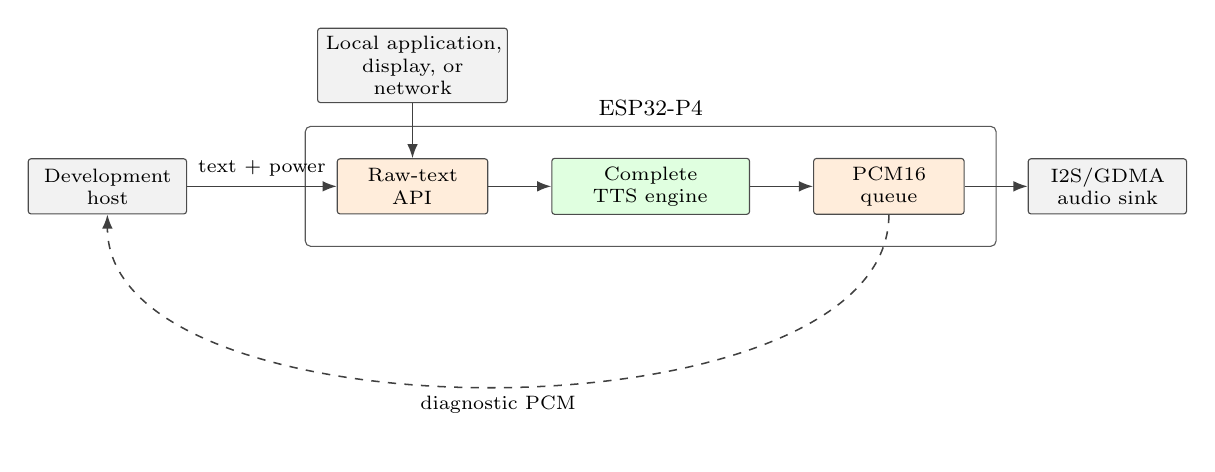
\begin{tikzpicture}[node distance=4mm and 8mm]
  \node[paperio, text width=18mm] (host) {Development\\host};
  \node[paperfw, text width=17mm, right=19mm of host] (api) {Raw-text\\API};
  \node[papersystem, text width=23mm, right=of api] (engine)
    {Complete\\TTS engine};
  \node[paperfw, text width=17mm, right=of engine] (queue) {PCM16\\queue};
  \node[paperio, text width=18mm, right=of queue] (sink)
    {I2S/GDMA\\audio sink};
  \node[paperio, text width=22mm, above=7mm of api] (local)
    {Local application,\\display, or network};

  \node[draw=black!65, rounded corners=2pt, inner sep=4mm,
    fit=(api)(engine)(queue), label={[font=\footnotesize]above:ESP32-P4}]
    (board) {};

  \draw[paperarrow] (host) -- node[above, font=\scriptsize]
    {text + power} (api);
  \draw[paperarrow] (local) -- (api);
  \draw[paperarrow] (api) -- (engine);
  \draw[paperarrow] (engine) -- (queue);
  \draw[paperarrow] (queue) -- (sink);
  \draw[paperdash] (queue.south) to[out=-90,in=-90,looseness=0.75]
    node[midway, below, font=\scriptsize] {diagnostic PCM} (host.south);
\end{tikzpicture}
\caption{System boundary. USB is a development transport and power source;
phonemes, tokens, latent tensors, and waveform samples are produced inside
the ESP32-P4. A standalone application can call the same raw-text API and
send PCM to an I2S/GDMA sink.}
\label{fig:system-boundary}
\end{figure}

The work makes four contributions.

\begin{itemize}
  \item It documents a complete raw-text neural TTS deployment on an
  ESP32-P4, including the frontend, stochastic latent construction, flow,
  decoder, and audio conversion.
  \item It gives measured implementations for model and runtime problems that
  are hidden by parameter count: lowering transposed convolution, Conv1D
  scheduling, repeated layout conversion, mixed precision, and fixed-shape
  routing.
  \item It defines an evidence procedure that separates graph execution,
  integer parity, transport integrity, and audible speech quality. Several
  faster candidates had valid checksums and failed listening tests. The gates
  therefore remain separate.
  \item It reports flash, PSRAM, internal-memory, stack, latency, and static
  shape limits for a reproducible board and software revision.
\end{itemize}

The measured exact-weight runtime is slower than real time. This paper makes
no conversational or native-streaming claim. The practical result is a
complete local speech engine for short values, menu items, status messages,
navigation cues, and bounded queued announcements. The same port also gives a
measured starting point for later decoder training and causal synthesis work.

\section{Related Work}

\subsection{End-to-end neural speech synthesis}

VITS combines a text encoder, duration modeling, variational latent
variables, normalizing flows, and adversarial waveform generation in a single
training system \cite{kim2021vits}. Inflect follows this broad inference
structure and packages a complete fixed-voice text-to-waveform model. Its
release API supports CPU, CUDA, and ONNX execution, but the published
deployment interface returns complete waveform chunks and has no streaming
state \cite{song2026inflectdeployment,song2026inflectonnx}.

The waveform generator belongs to the family popularized by HiFi-GAN, where
transposed convolutions increase temporal resolution and multi-receptive-field
residual blocks refine the signal \cite{kong2020hifigan}. Such generators are
parallel on server hardware. Their long low-channel convolutions can be a poor
fit for an MCU because activations grow to waveform rate while cache and SIMD
width remain constrained.

Alternative vocoders reduce this cost through model design. LPCNet combines
linear prediction with a sparse recurrent network \cite{valin2019lpcnet}, and
later work reduced its cost further \cite{valin2022shoestring}. FARGAN
generates small subframes and uses long-term pitch prediction at a reported
600 MFLOP/s \cite{valin2024fargan}. Vocos predicts Fourier coefficients
instead of constructing a waveform through a deep time-domain upsampler
\cite{siuzdak2024vocos}. MB-iSTFT-VITS replaces part of a VITS waveform path
with inverse STFT and reports a 4.1-fold CPU synthesis speedup in its setting
\cite{kawamura2023mbistftvits}. These designs provide directions for a future
trained decoder. They cannot replace the released Inflect weights without a
new training and quality evaluation cycle.

\subsection{Neural inference on microcontrollers}

MCUNet showed that architecture and runtime have to be designed together
under MCU memory constraints \cite{lin2020mcunet}. TinyVocos applies this idea
to vocoding: its authors evaluated several purpose-built models on four MCUs
and report a best footprint of 1.5 MiB flash and 517 KiB RAM with MOS 3.95
\cite{ciapponi2024tinyvocos}. TinyVocos receives acoustic features and does not
provide the complete raw-text path evaluated here, but it establishes that a
modern neural vocoder can fit MCU-class resources.

ESP-DL provides quantized operators, a static memory planner, FlatBuffer-based
model files, and dual-core execution for Espressif chips
\cite{espressif2026espdl}. Its general operator set made the current port
possible. The installed implementation was oriented toward Conv2D scheduling;
the time dimension of a rank-three Conv1D tensor did not use both cores. The
runtime modifications described in Section~\ref{sec:runtime} address the
specific shapes of this speech decoder.

\section{Target System}

\subsection{Hardware and software freeze}

All board measurements were taken on one connected ESP32-P4 revision 1.3.
This early revision was configured at its supported 360 MHz frequency. The
module exposes 32 MiB of in-package hexadecimal PSRAM at 200 MHz and 16 MiB
of external flash. Table~\ref{tab:platform} gives the state used for the final
route. ESP32-P4 includes processor extensions and image/audio peripherals,
but it does not contain a neural processing unit \cite{espressif2026p4}.

\begin{table}[t]
\centering
\caption{Measured platform and pinned software.}
\label{tab:platform}
\small
\begin{tabularx}{\linewidth}{@{}lY@{}}
\toprule
Item & Exact state \\
\midrule
SoC & ESP32-P4 revision 1.3, two high-performance RISC-V cores at 360 MHz \\
Memory & 32 MiB in-package PSRAM, hexadecimal mode, 200 MHz \\
Flash & 16 MiB, 80 MHz DIO in the tested configuration \\
Inference SDK & ESP-IDF 6.0.2 and ESP-DL 3.3.9 \\
Exporter & ESP-PPQ 1.3.7, ONNX 1.17.0, Python 3.12.11 \\
Model & \texttt{owensong/Inflect-Nano-v2}, revision \texttt{1cbf8079...} \\
Checkpoint & 15,971,083 B; SHA-256 \texttt{bfca4684...25b3} \\
Frontend & eSpeak-NG 1.52.0, commit \texttt{4870adfa...d6c} \\
Output & 24 kHz, mono, signed PCM16 little-endian \\
\bottomrule
\end{tabularx}
\end{table}

The software state was frozen before graph changes. The Hugging Face snapshot,
model checkpoint, configuration, ESP-DL component, exporter environment, and
host golden tensors were identified by commit or SHA-256. Version pinning was
necessary because graph layout and per-channel quantization behavior changed
across ESP-DL and ESP-PPQ releases. Historical exports made with ESP-PPQ 1.3.6
remain reproducible evidence; new final-route exports use 1.3.7.

\subsection{Model decomposition}

The checkpoint contains 3,966,721 parameters before release-time weight-norm
removal and 3,958,801 active parameters after removal. The waveform decoder
contains 2,092,368 active parameters. We split inference into an embedding
table, an acoustic graph, deterministic MCU glue, an inverse-flow graph, and
a waveform decoder. Table~\ref{tab:modelparts} records the learned parts.

Figure~\ref{fig:pipeline} gives the complete data path and distinguishes
learned ESP-DL graphs from deterministic firmware stages. This distinction
was required for memory accounting and parity tests.

\begin{figure}[t]
\centering
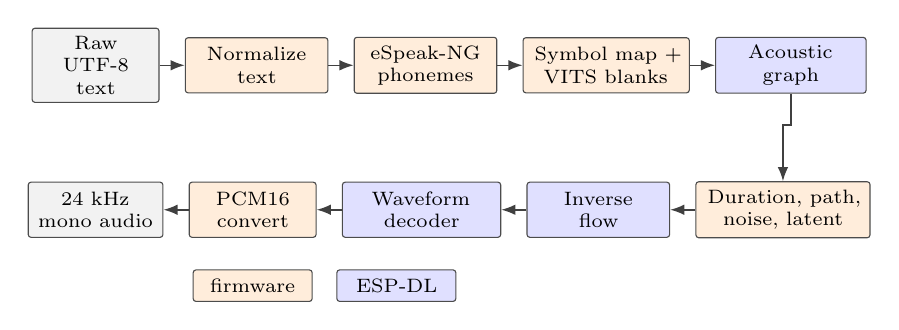
\begin{tikzpicture}[node distance=4mm and 3.2mm]
  \node[paperio, text width=14mm] (text) {Raw UTF-8\\text};
  \node[paperfw, text width=16mm, right=of text] (norm)
    {Normalize\\text};
  \node[paperfw, text width=16mm, right=of norm] (espeak)
    {eSpeak-NG\\phonemes};
  \node[paperfw, text width=19mm, right=of espeak] (tokens)
    {Symbol map +\\VITS blanks};
  \node[paperlearned, text width=17mm, right=of tokens] (acoustic)
    {Acoustic\\graph};

  \node[paperio, text width=15mm, below=10mm of text] (audio)
    {24 kHz\\mono audio};
  \node[paperfw, text width=14mm, right=of audio] (pcm) {PCM16\\convert};
  \node[paperlearned, text width=18mm, right=of pcm] (decoder)
    {Waveform\\decoder};
  \node[paperlearned, text width=16mm, right=of decoder] (flow)
    {Inverse\\flow};
  \node[paperfw, text width=20mm, right=of flow] (glue)
    {Duration, path,\\noise, latent};

  \draw[paperarrow] (text) -- (norm);
  \draw[paperarrow] (norm) -- (espeak);
  \draw[paperarrow] (espeak) -- (tokens);
  \draw[paperarrow] (tokens) -- (acoustic);
  \draw[paperarrow] (acoustic.south) -- ++(0,-4mm) -| (glue.north);
  \draw[paperarrow] (glue) -- (flow);
  \draw[paperarrow] (flow) -- (decoder);
  \draw[paperarrow] (decoder) -- (pcm);
  \draw[paperarrow] (pcm) -- (audio);

  \node[paperfw, minimum height=4mm, text width=13mm,
    below=4mm of pcm] (fwlegend) {firmware};
  \node[paperlearned, minimum height=4mm, text width=13mm,
    right=3mm of fwlegend] (mllegend) {ESP-DL};
\end{tikzpicture}
\caption{Complete on-device text-to-waveform path. Orange blocks are explicit
firmware or the embedded eSpeak frontend; blue blocks are learned graphs
executed by ESP-DL. USB does not perform any stage in this path.}
\label{fig:pipeline}
\end{figure}

\begin{table}[t]
\centering
\caption{Learned inference decomposition. Parameter counts refer to the active
deployment graph after weight-norm removal.}
\label{tab:modelparts}
\small
\begin{tabularx}{\linewidth}{@{}lrrY@{}}
\toprule
Part & Parameters & Primary shape & Function \\
\midrule
Embedding & 12,816 & $178\times72$ & Token ID to quantized text embedding \\
Acoustic core & 837,297 & $T_{text}\leq49$ & Text encoding, statistics, and durations \\
Inverse flow & 1,016,320 & $128\times T_z$ & Prior latent to decoder latent \\
Waveform decoder & 2,092,368 & $128\times T_z$ & 256 PCM samples per latent frame \\
\bottomrule
\end{tabularx}
\end{table}

At runtime, normalized text becomes phoneme tokens $x$. The acoustic graph
returns latent statistics and log durations. Firmware applies the released
duration exponentiation, speed scaling, ceiling, and bounds, then constructs
the monotonic token-to-latent path. Means and log scales are expanded along
that path. A pinned standard-normal noise tensor, seed, and variation control
produce the prior latent $z_p$. Four inverse coupling blocks map $z_p$ to the
decoder latent $z$. The waveform generator expands each latent frame by a
factor of 256 and returns a mono waveform.

Several operations remain in C++ instead of a learned graph. Embedding lookup
is a bounded table access. Mask construction, duration rounding, monotonic
path construction, latent expansion, noise combination, tensor-layout
conversion, PCM conversion, and checksums are simpler and smaller as explicit
firmware code. A local floating-point \texttt{Where} module fills one gap in
the installed ESP-DL operator set.

\subsection{Waveform decoder structure}

The active release decoder receives $[B,128,T_z]$. A $7$-tap convolution maps
128 channels to 192. Four transposed convolutions then upsample by
$8,8,2,2$ while reducing channels to $96,48,24,12$. Each stage averages three
residual branches with kernel sizes 3, 7, and 11; each branch uses dilation
pairs derived from 1, 3, and 5. A final leaky activation, $7$-tap convolution,
and hyperbolic tangent produce the waveform. The graph contains 74 ordinary
Conv1D operations, four ConvTranspose1D operations, and twelve residual
blocks.

For a 96-frame input, the decoder performs 4,159,143,936 nominal MACs and
emits 24,576 samples, or 1.024 s. This is 4.062 GMAC per second of output
audio. The $k=11$ residual branches account for 50.54\% of decoder MACs;
$k=7$ branches account for 32.16\%, and $k=3$ branches account for 13.78\%.
The pre/post convolutions and four upsamplers together account for about
3.52\%. The decoder is small in parameter bytes and expensive in repeated
time-domain arithmetic.

An analytic dependency trace and direct zero-padding checks found 13 latent
frames of context on each side of an interior output region. The complete
dependency span is 27 frames. Since each frame represents 256 samples, one
side of context equals

\begin{equation}
  \frac{13\cdot256}{24000}=138.667\ \mathrm{ms}.
\end{equation}

This context determines safe bucket routing and rules out zero-lookahead exact
streaming with the released weights.

\section{Porting Method}

\subsection{Reference-first procedure}

The port was developed as a sequence of falsifiable stages. A deterministic
host canary, \texttt{Testing one two three.} with seed 17, produced input
tokens, the latent entering the decoder, intermediate tensors, the float
waveform, and hashes. Operator feasibility was measured before the complete
graph was exported. Each graph rewrite had to pass a float comparison before
quantization, the ESP-PPQ host executor after quantization, and the ESP-DL
embedded test vector on the board.

The first real-layer gate used all 27,456 outputs of the decoder pre-
convolution. It exposed two deployment details. ESP-PPQ packs P4 filters in
16-channel blocks rather than ordinary contiguous PyTorch order, and the P4
kernel uses round-half-to-even during accumulator shifts. Implementing both
rules produced zero integer mismatches for per-tensor and per-channel weight
quantization. This layer gate prevented graph-level audio errors from being
misdiagnosed as model-quality problems.

\subsection{Exact polyphase transposed convolution}
\label{sec:polyphase}

The initial ESP-PPQ lowering of \texttt{ConvTranspose1d} inserted zeros before
an ordinary convolution. For the first $k=16$, stride-8 upsampler, this
executed about 337 million MACs in place of the 42.17 million logical MACs.
The upsample convolution alone took about 2.6 s on the board.

We replaced every transposed convolution with an exact polyphase form. A
stride-$s$ transposed convolution can be separated into $s$ ordinary
convolutions, one for each output phase. The phase outputs are interleaved in
time after any exponent alignment. The two $k=16$, stride-8 layers use eight
two-tap phases; the two $k=4$, stride-2 layers use two two-tap phases. No
zero-filled activation is materialized.

Figure~\ref{fig:polyphase} contrasts the exported zero-insertion graph with
the exact implementation used on the board. Both routes implement the same
linear operator; the second executes only the nonzero phases.

\begin{figure}[t]
\centering
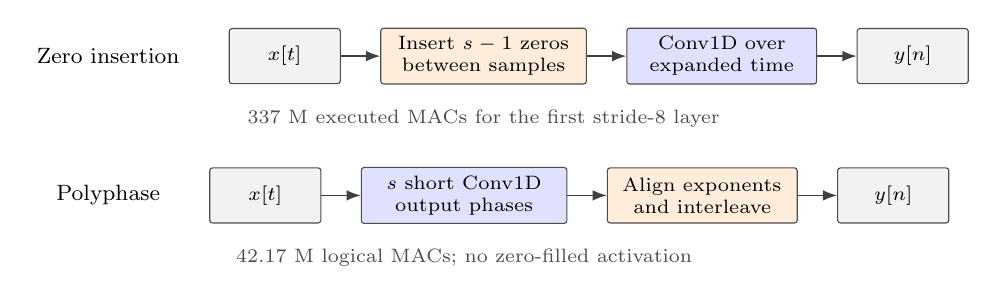
\begin{tikzpicture}[node distance=4mm and 5mm]
  \node[font=\footnotesize, anchor=east] (naivelabel) at (0,0)
    {Zero insertion};
  \node[paperio, text width=12mm, right=of naivelabel] (nx) {$x[t]$};
  \node[paperfw, text width=24mm, right=of nx] (zeros)
    {Insert $s-1$ zeros\\between samples};
  \node[paperlearned, text width=22mm, right=of zeros] (longconv)
    {Conv1D over\\expanded time};
  \node[paperio, text width=12mm, right=of longconv] (ny) {$y[n]$};

  \node[font=\footnotesize, anchor=east, below=13mm of naivelabel]
    (phaselabel) {Polyphase};
  \node[paperio, text width=12mm, right=of phaselabel] (px) {$x[t]$};
  \node[paperlearned, text width=24mm, right=of px] (phases)
    {$s$ short Conv1D\\output phases};
  \node[paperfw, text width=22mm, right=of phases] (align)
    {Align exponents\\and interleave};
  \node[paperio, text width=12mm, right=of align] (py) {$y[n]$};

  \draw[paperarrow] (nx) -- (zeros);
  \draw[paperarrow] (zeros) -- (longconv);
  \draw[paperarrow] (longconv) -- (ny);
  \draw[paperarrow] (px) -- (phases);
  \draw[paperarrow] (phases) -- (align);
  \draw[paperarrow] (align) -- (py);

  \node[font=\scriptsize, text=black!70, below=2mm of zeros]
    {$337$ M executed MACs for the first stride-8 layer};
  \node[font=\scriptsize, text=black!70, below=2mm of phases]
    {$42.17$ M logical MACs; no zero-filled activation};
\end{tikzpicture}
\caption{Exact polyphase lowering of transposed convolution. The original
export expanded time with zeros before convolution. The deployed graph
computes one short convolution per output phase and interleaves the results.}
\label{fig:polyphase}
\end{figure}

The complete transformed FP32 decoder differed from the release decoder by
$5.49\times10^{-8}$ mean absolute error and $2.97\times10^{-6}$ maximum
absolute error on the fixed latent. Correlation was
$0.999999999996$. On the first complete residual stage, polyphase lowering
reduced board time from 3.493 s to 1.366 s, a 2.557-fold speedup, with zero
integer mismatches after quantization.

The initial implementation built the interleave from portable slice, concat,
reshape, and transpose operators. A later custom fused interleave was measured
on all four real shapes. It reduced that layout chain from 101.120 ms to
78.967 ms. The projected whole-decoder gain was only 0.772\%, so the custom
operator was not included in the final graph. This test prevented a visually
large graph rewrite from consuming further effort after its measured upper
bound became small.

\subsection{Quantization and audible output precision}

ESP-PPQ exports power-of-two quantization compatible with ESP-DL. Convolution
weights use symmetric per-output-channel scales, while ordinary activations
use symmetric per-tensor scales. Integer-only inference follows the usual
affine-quantization principles \cite{jacob2018integer}, with the target's
packing and rounding behavior included in parity tests.
The exporter version and its target-specific dispatch are pinned separately
from the firmware runtime \cite{espressif2026espppq}.

The first complete decoder used INT8 throughout and returned an INT8 waveform
with exponent $-8$. Its WAV container was PCM16, although every sample was a
multiple of 128. A valid board utterance used only 121 distinct sample levels.
Direct listening found stable background noise. Quantizing only a clean FP32
waveform to the same final step gave 35.29 dB SNR and 0.999852 correlation;
the complete INT8 graph gave 4.11 dB SNR and 0.789805 correlation. Error had
already accumulated before the final output quantizer.

Layerwise analysis identified the input convolution and first upsampling
stage as sensitive. Three mixed-precision candidates were exported. Promoting
individual residual convolutions introduced a precision boundary inside a
residual path and worsened error. Promoting the input convolution and first
upsampling pair improved correlation from 0.790 to 0.824. Extending INT16 to
the final convolution and tanh produced an INT16 output at exponent $-16$
with 6,120 distinct levels and a nonzero-value greatest common divisor of 1
on the board. This \texttt{mixed-front-head} route increased the 96-frame
decoder time by 6.1\% relative to all INT8. It was retained because direct
listening preferred its usable output precision and because the remaining
memory was ample.

Waveform statistics were treated as diagnostics. Correlation, SNR, RMS,
clipping, and unique levels can locate a quantization failure; none establishes
intelligibility or naturalness. The experiment therefore allowed a changed
PCM hash after a declared quantization change and required direct listening to
the exact board artifact.

\subsection{ESP-DL runtime changes}
\label{sec:runtime}

Inspection of the installed ESP-DL source found that multi-core Conv2D divided
work along input height. Conv1D tensors were represented with height one and
time along width, so this path could not divide speech convolutions between
cores. A narrow Conv1D path now splits the output time axis. Each core receives
one output interval and only the input overlap required by the dilated kernel.
Outer padding is applied at the corresponding end. Quantization metadata
ownership remains with the original runtime argument.

At 512 KiB L2 cache, the custom single-core decoder took 8.630 s and the
dual-core path took 5.037 s, a 1.713-fold gain with identical 36,608-byte INT8
output. The gain is below two because both cores share the PSRAM/cache path and
some operators remain serial.

The stock graph also spent seconds moving between channel-first and
channel-last layouts. A specialized transpose handles the common
$[0,2,1]$ permutation as tiled contiguous copies and divides large copies
between cores. Two graph passes then reduced the number of transfers. The
first deduplicates post-layout transpose fan-outs only when shape, data type,
exponent, layout, permutation, and target platform match. It removed twelve
operations and reduced a padded decoder by 142.4 ms. The second propagates
native NWC layout through compatible slice paths and removed eight more
transpose nodes.

Late decoder stages use 24 and 12 channels, which underfill the P4 vector
kernels. Padding these stages to 32 and 16 channels, while maintaining zeros
in added channels across convolution, activation, residual addition, and
output cropping, reduced the decoder from 5.578 s to 3.971 s. The output
remained byte-identical. This trade spent about 1.25 MiB of additional PSRAM
to reduce execution by 28.8\%.

Activation profiling showed 69 leaky-ReLU lookup tables. Exhaustive inspection
of every signed INT8 input reduced them to seven exact formula classes. A P4
SIMD implementation applies the corresponding scale, negative slope,
round-half-to-even shift, and small correction masks for decimal slopes. All
138 tables across two decoder buckets matched for all 256 inputs. The formula
path reduced the full decoder by 42.3 ms and the 96-frame decoder by 27.4 ms.
Unrecognized tables keep the generic ESP-DL lookup implementation.

Several apparently useful changes were rejected by direct board A/B tests.
Dual-core flat additions and requantization increased PSRAM traffic and slowed
the graph. A larger ESP-DL tensor-planner allocation consumed scarce internal
RAM for less than a 0.3\% latency change. Executing parameters from flash saved
2.13 MiB PSRAM but made inference 27.4\% slower. These results illustrate why
operator count and isolated kernel speed did not predict the final runtime.

\subsection{Resident service and model buckets}

Repeated model construction added more than one second to each request. The
command service verifies the model package once at boot, constructs model
objects on first use, and keeps them resident. A historical 143-frame route
dropped from 5.336 s for the first request to 3.789 s when warm, while the
learned arithmetic remained near 3.53 s.

Static decoder shapes wasted work on zero padding. A 143-frame decoder took
about 2.96 s whether a phrase required 71, 74, or 106 frames. We exported a
96-frame decoder and proved that its output equals the first 83 valid frames
of a zero-padded 143-frame graph. The remaining 13 frames are right context.
For \texttt{Good morning.}, selecting T96 reduced the decoder from 2.962 s to
2.073 s. The later accepted mixed-precision and runtime path measured about
2.013 s.

The final short-value package adds a T64 decoder. T64 has a 51-frame safe
prefix after reserving right context. The measured \texttt{Ready.} request
requires 44 frames, so T64 replaces T96 for this case and reduces decoder time
from 2.013 s to 1.335 s. The complete residual structure remains intact.

\begin{figure}[t]
\centering
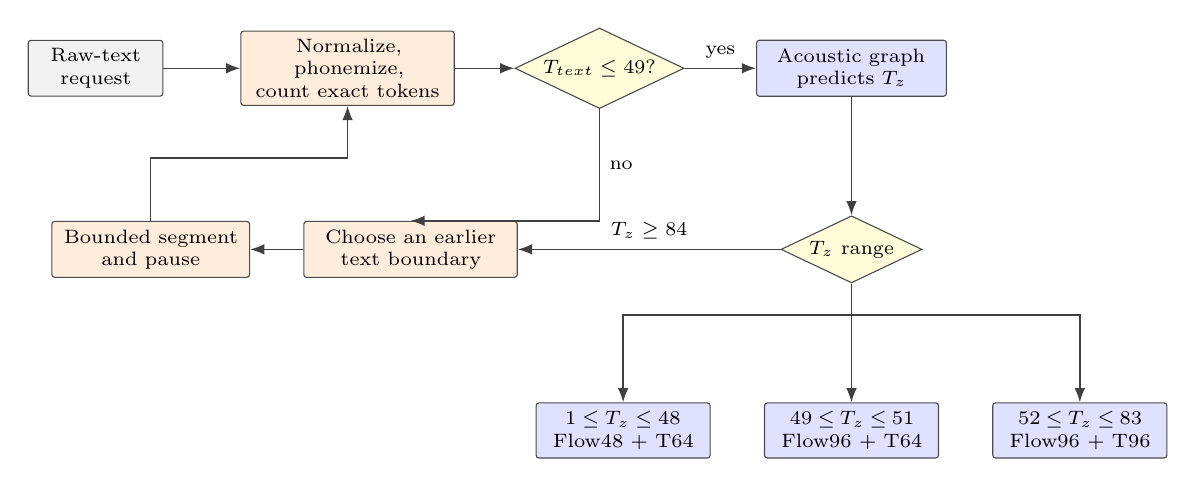
\begin{tikzpicture}[x=1mm,y=1mm]
  \node[paperio, text width=15mm] (request) at (5,38)
    {Raw-text\\request};
  \node[paperfw, text width=25mm] (frontend) at (37,38)
    {Normalize, phonemize,\\count exact tokens};
  \node[paperdecision] (tokengate) at (69,38)
    {$T_{text}\leq49$?};
  \node[paperlearned, text width=22mm] (acousticroute) at (101,38)
    {Acoustic graph\\predicts $T_z$};

  \node[paperfw, text width=25mm] (planner) at (45,15)
    {Choose an earlier\\text boundary};
  \node[paperfw, text width=23mm] (segment) at (12,15)
    {Bounded segment\\and pause};
  \node[paperdecision] (bucket) at (101,15) {$T_z$ range};

  \node[paperlearned, text width=20mm] (routea) at (72,-8)
    {$1\!\leq\!T_z\!\leq\!48$\\Flow48 + T64};
  \node[paperlearned, text width=20mm] (routeb) at (101,-8)
    {$49\!\leq\!T_z\!\leq\!51$\\Flow96 + T64};
  \node[paperlearned, text width=20mm] (routec) at (130,-8)
    {$52\!\leq\!T_z\!\leq\!83$\\Flow96 + T96};

  \draw[paperarrow] (request) -- (frontend);
  \draw[paperarrow] (frontend) -- (tokengate);
  \draw[paperarrow] (tokengate) -- node[above, font=\scriptsize] {yes}
    (acousticroute);
  \draw[paperarrow] (tokengate.south) |- node[pos=0.25, right,
    font=\scriptsize] {no} (planner.north);
  \draw[paperarrow] (acousticroute) -- (bucket);
  \draw[paperarrow] (bucket) -- node[above, font=\scriptsize]
    {$T_z\geq84$} (planner);
  \draw[paperarrow] (planner) -- (segment);
  \draw[paperarrow] (segment.north) -- ++(0,8mm) -| (frontend.south);
  \draw[paperarrow] (bucket.south) -- ++(0,-4mm) -| (routea.north);
  \draw[paperarrow] (bucket.south) -- (routeb.north);
  \draw[paperarrow] (bucket.south) -- ++(0,-4mm) -| (routec.north);
\end{tikzpicture}
\caption{Shape-aware dispatcher and bounded long-text fallback. Token count
is checked with the actual embedded frontend, while latent length is checked
after duration prediction. Requests that exceed either static limit return to
a valid text boundary before buffers are allocated.}
\label{fig:routing}
\end{figure}

\noindent\begin{minipage}{\linewidth}
\setlength{\parindent}{1em}
Reverse flow had the same fixed-shape waste. Flow96 took about 465 ms for the
44-frame request. A Flow64 export reduced it to 308.3 ms. Flow48 reduced it to
234.6 ms and preserved exact FP32 valid-region equality against the masked
143-frame graph. Figure~\ref{fig:routing} shows the current dispatcher and
the segmentation loop that precedes flow and decoder selection.
\end{minipage}

The route keeps flow and decoder limits independent. Flow96 occupies a
separate 2 MiB flash partition; the main model package contains the acoustic
model, Flow48, T64, and T96. Adding every historical model was rejected because
it would exceed the 16 MiB flash device and retain unreachable choices.

\subsection{On-device raw-text frontend}

The release frontend normalizes English text and uses eSpeak-NG to produce
North American English phonemes with stress and punctuation. The port embeds
the exact eSpeak-NG 1.52.0 source \cite{espeakng2026}. A read-only 1 MiB FAT
partition holds a stripped English voice, dictionary, phoneme tables, and
intonation data. The full multi-language host data package was excluded.

The board frontend performs UTF-8 and punctuation normalization, release-
specific word overrides, phonemization, lookup in the exact model symbol
order, blank insertion, and bounds checking. The C++ normalizer implements
the released order of money, date, time, phone, version, decimal, ordinal,
number, acronym, punctuation, and model-specific rules without Python or
regular expressions.

eSpeak exposed an internal-memory problem that model-only profiling would not
find. A 16 KiB task stack overflowed; measured use exceeded 40 KiB. The final
implementation creates a temporary worker with a 48 KiB internal-RAM stack,
waits for completion, synchronously deletes the task, and frees its task
control block and stack before neural inference. A dynamic-task version relied
on deferred idle-task cleanup and reduced the largest free internal block to
31,744 bytes, preventing a second call. Explicit lifetime management restores
the 63,488-byte largest block.

The stack cannot reside in PSRAM because eSpeak accesses flash-backed data and
ESP-IDF forbids a PSRAM task stack on paths that can run while flash cache is
disabled. Integration also found an unaligned embedded float asset. Replacing
the generated embedded-file section with a four-byte-aligned assembly include
placed the asset at a verified address ending in \texttt{518} and removed the
fault.

The board passed nine release-parity cases. For every case, normalized text,
IPA, each token ID, and token FNV-1a matched the pinned Python frontend. The
corpus covers ordinary text, money, dates, time, identifiers, phone suffixes,
versions, decimals, ordinals, long numbers, acronyms, street abbreviations,
punctuation, and release-specific names. Board frontend time ranged from
2.455 to 6.099 ms with a mean of 3.839 ms. This cost is negligible relative
to the learned path.

\subsection{Bounded long-text planning}

The static acoustic graph accepts at most 49 frontend tokens. Blank insertion
means character count is a poor proxy, especially after number and date
normalization. The firmware normalizes the complete input once and then asks
the real board frontend to evaluate candidate boundaries. It prefers sentence
boundaries, then sufficiently late clause punctuation, then whitespace. It
never splits a UTF-8 sequence, a decimal point between digits, a word, a
phoneme, or a token vector. An individual word that exceeds the bound returns
an explicit error.

Each planned segment stores its source text, synthesis text, normalized text,
phonemes, token IDs, boundary class, and following pause. The acoustic graph
provides a second sizing gate: exact predicted durations are summed before the
latent, flow, decoder, or PCM buffers are allocated. A typed duration overflow
contains required and available frame counts. The planner can then move to an
earlier word boundary. Runtime limits cap a request at 64 segments and 32
duration replans.

A narrow punctuation rescue avoids a one-word tail when only terminal
punctuation exceeds 49 tokens. It may remove one final punctuation symbol from
the synthesis text while preserving the original source boundary and pause in
telemetry. Internal punctuation and punctuation on a fitting request remain
unchanged.

The board verified planner decisions for short values, two sentences,
normalized decimals, late comma selection, whitespace fallback, closing quote
direction, and an oversized word. Successful segments contained at most 49
tokens; the longest planner-only request took 59.114 ms. A complete segmented
request produced independently framed PCM segments, edge fades, and boundary
silence. The host verified each segment before concatenating a listening WAV.
The intended device implementation sends the same bounded segment directly to
I2S/GDMA and reuses its inference buffers.

Long-text support bounds memory and preserves words. It does not carry prosody
state across segments, and it cannot guarantee gap-free playback while the
decoder is slower than real time. The suitable output is a sequence of short
announcements rather than continuous narration.

\section{Experimental Method}

\subsection{Measurement boundaries}

Timers were placed around model loading, every learned graph, MCU glue, and
the complete request. Binary PCM transmission begins after the inference
timer. Reported model latency therefore excludes host-side WAV creation and
serial transfer. Cold measurements include first model construction only when
explicitly labeled. Warm measurements reuse resident objects.

Real-time factor is

\begin{equation}
  \mathrm{RTF}=\frac{t_{compute}}{N_{samples}/24000},
\end{equation}

where values above one are slower than playback. ``Time to first audio'' for
the current graph equals the time to the complete PCM buffer because the
decoder has no output callback or persistent streaming state.

The experiment did not collect large repeated timing distributions for every
minor change. Each hypothesis used the cheapest board test that could change
the implementation decision. Repeated runs were added when transport,
scheduler variation, or a near-threshold result made a decision ambiguous.

\subsection{Evidence hierarchy}

Four forms of evidence answer different questions.

\begin{enumerate}
  \item Float graph comparison verifies that a mathematical rewrite preserves
  the release model before quantization.
  \item ESP-PPQ and embedded ESP-DL vectors verify quantized integer execution.
  The strongest parity tests compare every output element.
  \item Framing, byte counts, board and host FNV-1a, PCM SHA-256, and WAV-header
  checks verify that captured audio is exactly what the board emitted.
  \item Direct listening checks intelligibility, voice, stable noise, ending
  completion, and segmentation boundaries.
\end{enumerate}

Passing an earlier level does not imply a later one. During development, a
tiled decoder combined with reverse-flow pruning produced valid shapes,
stable timings, correct checksums, and unintelligible noise. An earlier stack
of runtime branch removals did the same. Both were rejected. The accepted
control disabled all unvalidated pruning and tiling, reproduced an already
heard short waveform byte for byte, and became the base for T64 and Flow48.

\subsection{Audio transport}

Early captures encoded PCM as hexadecimal UART records, doubling data size and
making a 71 kB waveform take more than twelve seconds at 115200 baud. The
persistent service uses framed binary PCM at 460800 baud. Each frame declares
its byte count and ends with a board checksum. The host rejects a short or
corrupt payload and retries transport only; frontend or inference failures are
returned unchanged.

The CH340 serial bridge still lost bytes in a small number of large transfers.
Splitting writes into 2 KiB pieces and waiting for UART completion improved
capture reliability. This transport does not influence measured graph time.
I2S/GDMA is the appropriate local audio sink because 24 kHz mono PCM16 requires
only 48 kB/s and avoids diagnostic round trips.

\section{Results}

\subsection{First complete waveform and full pipeline}

The first complete decoder accepted the real $[1,128,143]$ latent from the
host golden and produced 36,608 samples. ESP-DL matched all 36,608 embedded
INT8 outputs with maximum integer error zero. Decoder execution took 12.809 s
for 1.525 s of audio, an RTF of 8.398. Model allocation was 245.59 KiB internal
RAM and 5,153.09 KiB PSRAM. After model destruction, free PSRAM returned to its
pre-load value.

The next milestone ran embedding, acoustic inference, duration/path/noise
glue, inverse flow, decoder, and PCM conversion on the board. For
\texttt{Testing one two three.}, the board produced 35,584 samples, or
1.482667 s. Board and host byte counts, chunk order, FNV-1a, PCM SHA-256, and
the WAV header passed. The initial learned stages took 6.138 s, including
5.578 s in the decoder. A cold request took 7.411 s because models were loaded
sequentially.

Table~\ref{tab:progression} summarizes the main runtime changes. Rows after
the first three include graph, quantization, or shape changes and should be
read as deployment milestones rather than a single-factor ablation.

\begin{table*}[t]
\centering
\caption{Decoder optimization progression on the connected board. All rows
use release weights unless the row explicitly changes static shape or
precision.}
\label{tab:progression}
\small
\begin{tabularx}{\textwidth}{@{}lrrY@{}}
\toprule
Milestone & Decoder time & Audio geometry & Main mechanism \\
\midrule
First complete decoder & 12.809 s & T143, 1.525 s & Portable polyphase graph, stock scheduling \\
Stock graph, 512 KiB L2 & 10.078 s & T143, 1.525 s & Cache increase \\
Dual-core Conv1D and transpose & 5.037 s & T143, 1.525 s & Time-axis split and specialized layout copy \\
Late-channel padding & 3.971 s & T143, 1.483 s & 24/12 channels padded to 32/16 \\
Transpose fan-out CSE & 3.833 s & T143, 1.483 s & Twelve exact duplicate copies removed \\
Slice-layout and resident service & 2.986 s & T143, 1.483 s & NWC propagation and warm model objects \\
Final unpruned Full143 control & 2.824--2.827 s & Segmented controls & Formula LUT, tiled transpose, mixed precision \\
T96 accepted route & 2.013 s & Up to 83 valid frames & Short static decoder bucket \\
T64 accepted route & 1.335 s & Up to 51 valid frames & Short-value decoder bucket \\
\bottomrule
\end{tabularx}
\end{table*}

\subsection{Raw-text parity and synthesis}

Table~\ref{tab:frontend} gives four direct board frontend cases. The host sent
only the text in the first column. The full nine-case normalization suite also
matched every compared field.

\begin{table}[t]
\centering
\caption{On-device frontend parity examples.}
\label{tab:frontend}
\small
\begin{tabularx}{\linewidth}{@{}Yrrr@{}}
\toprule
Raw text & Tokens & Token hash & Time \\
\midrule
\texttt{Hello.} & 15 & \texttt{37b5b29c} & 2.361 ms \\
\texttt{Good morning.} & 29 & \texttt{55879e9c} & 3.549 ms \\
\texttt{Turn left.} & 25 & \texttt{132e7058} & 3.235 ms \\
\texttt{Hello from the board.} & 43 & \texttt{380c159f} & 3.377 ms \\
\bottomrule
\end{tabularx}
\end{table}

The \texttt{Room 12.} synthesis request exercised normalization rather than
the diagnostic frontend command. The board converted it to
\texttt{Room twelve.}, produced 27 exact tokens, and returned 19,712 PCM
samples, or 0.821333 s. Different raw inputs produced different token hashes,
predicted durations, sample counts, and PCM hashes, excluding replay of a
compiled waveform.

\subsection{Final short-value route}

The final connected-board gate used \texttt{Ready.}. It produced 44 latent
frames and 11,264 PCM samples, or 0.469333 s. Acoustic inference, Flow48, and
T64 together took 1.656448 s. Flow48 took 234.609 ms and T64 took 1.335012 s.
Flow48 reduced the learned path by 70.312 ms relative to Flow64 and by 12.104\%
relative to the earlier T64 plus Flow96 control. The current complete learned
path has RTF 3.530 and throughput 0.283 times real time for this request.

Board and host agreed on PCM FNV-1a \texttt{51971333}. The WAV SHA-256 is
\texttt{add6b5be...381b8}; direct listening confirmed the spoken word, voice,
and complete ending. This is a single acceptance gate, not a MOS study or a
latency distribution.

The route is faster for short device values because its runtime follows the
smallest valid static graph. A phrase such as \texttt{Battery low.} requires
80 frames and therefore uses Flow96 plus T96. Longer values may cross either
the 49-token acoustic limit or the 83-frame deployment limit and are segmented
at a text boundary.

\subsection{Flash and memory}

Table~\ref{tab:resources} records the final short-value build. The 16 MiB flash
layout has a 4 MiB factory application partition, a \texttt{0x820000}-byte
main model partition, a 1 MiB G2P partition, and a 2 MiB Flow96 partition.
About 852 kB remains after the last partition.

\begin{table}[t]
\centering
\caption{Final deployment resources after the relevant routes and frontend
have been exercised. Decimal MB is used for allocator byte counts.}
\label{tab:resources}
\small
\begin{tabularx}{\linewidth}{@{}Yr@{}}
\toprule
Resource & Measured value \\
\midrule
Application image & 1,933,440 B \\
Main four-member model package & 8,409,632 B \\
Flow96 package & 1,345,632 B \\
Fixed embedding/noise/token asset & 86,198 B \\
Free bytes in main model partition & 110,048 B \\
Free PSRAM & 17,539,168 B \\
Largest free PSRAM block & 17,301,504 B \\
Free internal RAM & 99,551 B \\
Largest free internal block & 63,488 B \\
Main service stack headroom & 13,296 B \\
\bottomrule
\end{tabularx}
\end{table}

PSRAM is sufficient for the complete resident service. Internal RAM is the
tighter product resource because it must also hold task stacks and any future
DMA descriptors, network state, TLS buffers, and peripheral drivers. The
512 KiB L2 cache setting improves inference and removes on-chip memory from the
heap. The final application retains a 64 KiB internal-memory reserve and
measures the largest contiguous block rather than relying on total free bytes.

The current flash package leaves little room in its main partition. This is a
deliberate final set of reachable routes rather than an archive of every tested
bucket. A product requiring OTA slots, additional languages, or multiple
voices would need a new partition table, external storage, smaller models, or
a different decoder architecture.

\subsection{Segmentation results}

The connected planner kept a short screen value as one segment, preserved a
sentence boundary between two statements, normalized a decimal before
splitting, selected a useful late comma, split an unpunctuated sentence only
at spaces, handled closing quotes, and rejected an over-budget single word.
The longest accepted segment used exactly 49 tokens.

A complete multi-segment board request generated each segment, inserted its
pause, returned framed PCM, and released bounded buffers for reuse. The final
three-piece plan for one test message used 49, 41, and 49 tokens. The combined
geometry was 96,544 samples, or 4.022667 s including pauses. An experimental
decoder/flow combination produced only noise despite valid checksums and was
rejected. Repeating the same plan with the unpruned exact-flow control preserved
every planned source segment and the complete output geometry. Its short-path
PCM was byte-identical to the previously heard baseline.

The automatic segmentation mechanism is therefore established at the text,
token, duration, memory, and transport levels. The available listening
evidence supports short independent values and the unpruned decoder control.
The final long control still needs a formal listening study, and the model
resets prosody at every segment. This distinction matters for publication:
bounded long input is implemented, while continuous expressive narration is
outside the present result.

\section{Failure Analysis}

\subsection{Checksums cannot certify speech}

Two optimization groups deleted decoder residual work at inference time, and
one composite route combined a shortened decoder with a pruned inverse flow.
The outputs were finite, non-silent, correctly sized, stable across runs, and
transported without corruption. Listening found stationary noise with no
intelligible words. The options were disabled in the accepted build.

This failure changed the experiment procedure. Approximate flow and decoder
changes are now isolated, and each receives its own listening artifact before
composition. A complete package cannot inherit quality acceptance from its
members when they were calibrated separately. Output hashes establish
reproducibility only within one declared graph and quantization state.

\subsection{Quantization boundaries matter}

Promoting a few sensitive residual convolutions to INT16 seemed attractive in
a layerwise report. It worsened complete waveform error because the precision
boundary fell inside a residual path. Promoting coherent front and output
regions worked better. This supports block-level mixed-precision decisions
for residual generators. Individual layer scores do not include the cost of
conversion and requantization at branch merges.

The first all-INT8 output also demonstrated a presentation hazard. A file can
be valid 16-bit PCM while its source tensor carries about eight effective
bits. Container bit depth and model output precision must be reported
separately.

\subsection{Static shapes trade flash for response time}

T64 and T96 reduce padded computation and preserve the released weights, but
each duplicates most decoder parameters. The same applies to Flow48 and
Flow96. Buckets consume flash and still return audio only after a complete
graph. A bank of additional static lengths would eventually exhaust flash
without producing native streaming. The final dispatcher uses two decoder
lengths because both correspond to measured device-language cases and fit the
available layout.

\subsection{Memory lifetimes extend beyond tensors}

The model fit in PSRAM early in the project. The difficult memory failures
came from an eSpeak worker stack, deferred task cleanup, internal allocator
fragmentation, cache allocation, model metadata, and an unaligned embedded
asset. Peak tensor estimates would not predict any of them. Reproducible MCU
speech deployment needs measurements of internal free memory, largest blocks,
worker stack high-water marks, resident model allocations, and state after
repeated calls.

\subsection{Serial output can distort perceived performance}

Hexadecimal PCM at 115200 baud made a complete run appear much slower than
inference. Binary framing and separate timers corrected the measurement, but
the USB-UART bridge remained capable of dropping bytes. The host checksum
turned silent corruption into an explicit transport failure. A local I2S sink
removes this issue and uses little bandwidth compared with inference.

\section{Streaming and Practical Use}

The current decoder evaluates a complete static tensor and exposes PCM after
its final operation. Bucketing lowers that wait for short utterances. It does
not provide a sequence of valid early waveform blocks. An exact interior tile
needs 13 latent frames of left and right context. If a valid tile contains
$C$ frames, it evaluates approximately $C+26$ frames, so small tiles incur a
large overlap tax. A 24-frame valid core evaluates 50 frames; a 64-frame core
evaluates 90.

Throughput is the stricter constraint. The final \texttt{Ready.} route produces
0.469 s of audio in 1.656 s of learned computation. Starting playback from an
early tile would eventually underrun. No buffering strategy can sustain
playback when average production remains below one second of audio per second
of wall time. A retrained causal or fixed-lookahead decoder, or an efficient
spectral/recurrent vocoder, is required for conversational streaming.

The measured engine still has practical uses. A display can request speech for
a selected value, menu item, timer, connection state, or sensor reading. The
application can start synthesis when a value becomes likely to be spoken and
play the completed short buffer on selection. A device can generate a bounded
announcement before playback, cache common phrases, or queue several
independent status messages. These cases benefit from local text handling,
privacy, deterministic assets, and the absence of a network service. They can
tolerate seconds of generation more easily than an interactive dialogue.

The system has one fixed male English voice. It does not provide voice
cloning, speaker selection, multilingual inference, SSML coverage, native
pitch control, or validated emergency/accessibility speech. eSpeak-NG is
licensed under GPL-3.0-or-later; distribution of a proprietary firmware needs
a licensing plan or a compatible replacement frontend. Inflect weights and
code use Apache-2.0, ESP-IDF uses Apache-2.0, and ESP-DL uses MIT. License
compatibility is part of deployment design, not a property of model weights
alone.

\section{Reproducibility}

The repository retains source changes, exporters, test scripts, firmware,
model packages, board logs, JSON summaries, and listening WAVs. The experiment
report records hypotheses, raw results, failures, and decisions in chronological
order. Each logically complete change is a separate Git commit.

The final main package is named \texttt{short64-flow48}. Its size is
8,409,632 bytes, file SHA-256 is
\nolinkurl{3a267b2310a36ad5cc561e5ac3da78ee89aec66fb3b4c7df3abbd43280304bb9},
and its internal package digest is
\nolinkurl{b3ffb16b34e180a040796727385500adc6ad721d64c3b0082fdad25479c843cb}.
The matching application SHA-256 is
\nolinkurl{50462fa0add9f59b68ca9b8e7adc8525e4eb4427d839405694652a101b9d1634}.
Flow48 alone has SHA-256
\nolinkurl{a5688f144d41e8c966583d4df72e6f58991e4004fe6906c8d39939385ccf1a68}.

The final short board artifact is stored with machine-readable telemetry. Its
WAV SHA-256 is
\nolinkurl{add6b5be3e21278a46837c5a0269cee9392bbf6dc6081327082797963fd381b8};
the corresponding JSON SHA-256 is
\nolinkurl{17e17cb633b26863ae7c990cae0e0529f4fcec9c5917ffdca7eaa8b21500ec31}.
The reverse-engineering manifest records every decoder convolution shape,
nominal MAC count, real activation statistics, parameter group, and receptive
field result. Its SHA-256 is
\nolinkurl{3572eb3b963bdc98c2460957457665f5f538bfb6cd715a5017b67651a12a9b17}.

Reproduction requires the early P4 revision or a deliberate retarget. The
checked-in defaults select revision 1.x and 360 MHz; a binary built with these
settings is not a revision-3.x image. Board timing also depends on 200 MHz
hexadecimal PSRAM, cache size, parameter-copy policy, compiler optimization,
and the local ESP-DL Conv1D, transpose, and activation changes.

\section{Limitations and Publication Scope}

The paper reports one physical board and one fixed English voice. There is no
formal MOS, MUSHRA, or multi-listener preference study for the embedded
outputs. Listening decisions were direct engineering gates. The upstream
model's published quality metrics describe its host FP32 release and cannot be
assigned to this mixed-precision P4 port.

Power draw, regulator and SoC temperature, long-duration throttling, network
coexistence, I2S playback, watchdog behavior under a full application, and
24-hour stability have not been measured. Internal RAM is low enough that a
network stack and audio DMA require a fresh budget. The current USB protocol
is a diagnostic adapter rather than a product interface.

The static acoustic graph accepts 49 tokens. Segmentation extends finite input
length by issuing independent bounded requests. It does not model prosody
across boundaries. Natural duration-overflow recovery is implemented and
bounded; the test corpus did not produce a normal phrase that triggered it
after the token gate, so that particular replan branch lacks connected-board
coverage.

Claims of priority should remain narrow. We did not find an official or open
Inflect-Nano-v2 deployment on ESP32-P4 during the literature and repository
search. Absence from a search is not proof that no private or unpublished port
exists. The publishable contribution is the documented complete system,
measured runtime work, and evidence procedure.

An arXiv systems report is justified by the complete deployment and the
operator-level findings. A stronger peer-reviewed submission would add a
public reproducibility release, several boards, controlled listener ratings,
power measurements, I2S playback, and comparisons against at least one
purpose-built MCU vocoder. Achieving faster-than-real-time generation with a
trained causal or spectral decoder would constitute a separate model result.

\section{Conclusion}

We deployed a complete raw-text neural speech synthesizer on an ESP32-P4.
Normalization, English phonemization, tokenization, acoustic inference,
duration and latent construction, inverse flow, waveform decoding, and PCM16
conversion execute on the microcontroller. The host supplies text and receives
diagnostics; it performs no speech computation.

The result depended on system work beyond model compression. Exact polyphase
upsampling removed wasteful zero insertion. Dual-core Conv1D scheduling,
channel padding, layout specialization, graph CSE, mixed precision, resident
models, and shape-aware routing reduced the first 12.809-second decoder to a
1.335-second T64 path for a 44-frame short value. The complete learned route
takes 1.656 seconds and fits with the frontend in the board's flash and PSRAM.
The accepted build retains recognizable, intelligible short speech and rejects
faster candidates that produced noise.

The current engine is a complete local TTS implementation for short device
speech and bounded announcements. Its decoder is slower than real time and
returns complete buffers. These limits are measured properties of the released
model and runtime, and they identify the next technical problem: a decoder
trained for MCU throughput and explicit streaming state.

\bibliographystyle{plain}
\bibliography{references}

\end{document}
